% -----------------------------------------------
% Template for SMAC SMC 2013
% adapted and corrected from the template for SMC 2012, which was adapted from that of SMC 2011
% further updated for TENOR 2015 and 2016
% -----------------------------------------------

\documentclass{article}
\usepackage{tenor2016}
%\usepackage{times}
\usepackage{ifpdf}
\usepackage[english]{babel}
%\usepackage{cite}

%%%%%%%%%%%%%%%%%%%%%%%% Some useful packages %%%%%%%%%%%%%%%%%%%%%%%%%%%%%%%
%%%%%%%%%%%%%%%%%%%%%%%% See related documentation %%%%%%%%%%%%%%%%%%%%%%%%%%
%\usepackage{amsmath} % popular packages from Am. Math. Soc. Please use the 
%\usepackage{amssymb} % related math environments (split, subequation, cases,
%\usepackage{amsfonts}% multline, etc.)
%\usepackage{bm}      % Bold Math package, defines the command \bf{}
%\usepackage{paralist}% extended list environments
%%subfig.sty is the modern replacement for subfigure.sty. However, subfig.sty 
%%requires and automatically loads caption.sty which overrides class handling 
%%of captions. To prevent this problem, preload caption.sty with caption=false 
%\usepackage[caption=false]{caption}
%\usepackage[font=footnotesize]{subfig}

\usepackage{verbatim}
\newenvironment{INScode}		{\vspace{-2mm}\small\verbatim}{\endverbatim\vspace{-2mm}}

\newcommand{\sExpr}{\emph{score expressions} }
\newcommand{\SExpr}{\emph{Score expressions} }
\newcommand{\lowTilde} 		{\textasciitilde}

%user defined variables
\def\papertitle{INScore expressions to compose symbolic scores}
\def\authors{G. Lepetit-Aimon \qquad D. Fober \qquad Y. Orlarey \qquad S. Letz}
\def\firstauthor{Gabriel Lepetit-Aimon}
\def\secondauthor{Dominique Fober}
\def\thirdauthor{Yann Orlarey}
\def\fourthauthor{Stéphane Letz}

% adds the automatic
% Saves a lot of ouptut space in PDF... after conversion with the distiller
% Delete if you cannot get PS fonts working on your system.

% pdf-tex settings: detect automatically if run by latex or pdflatex
\newif\ifpdf
\ifx\pdfoutput\relax
\else
   \ifcase\pdfoutput
      \pdffalse
   \else
      \pdftrue
\fi

\ifpdf % compiling with pdflatex
  \usepackage[pdftex,
    pdftitle={\papertitle},
    pdfauthor={\firstauthor, \secondauthor, \thirdauthor},
    bookmarksnumbered, % use section numbers with bookmarks
    pdfstartview=XYZ % start with zoom=100% instead of full screen; 
                     % especially useful if working with a big screen :-)
   ]{hyperref}
  %\pdfcompresslevel=9

  \usepackage[pdftex]{graphicx}
  % declare the path(s) where your graphic files are and their extensions so 
  %you won't have to specify these with every instance of \includegraphics
  \graphicspath{{./figures/}}
  \DeclareGraphicsExtensions{.pdf,.jpeg,.png}

  \usepackage[figure,table]{hypcap}

\else % compiling with latex
  \usepackage[dvips,
    bookmarksnumbered, % use section numbers with bookmarks
    pdfstartview=XYZ % start with zoom=100% instead of full screen
  ]{hyperref}  % hyperrefs are active in the pdf file after conversion

  \usepackage[dvips]{epsfig,graphicx}
  % declare the path(s) where your graphic files are and their extensions so 
  %you won't have to specify these with every instance of \includegraphics
  \graphicspath{{./figures/}}
  \DeclareGraphicsExtensions{.eps}

  \usepackage[figure,table]{hypcap}
\fi

%setup the hyperref package - make the links black without a surrounding frame
\hypersetup{
    colorlinks,%
    citecolor=black,%
    filecolor=black,%
    linkcolor=black,%
    urlcolor=black
}


% Title.
% ------
\title{\papertitle}

% Authors
% Please note that submissions are NOT anonymous, therefore 
% authors' names have to be VISIBLE in your manuscript. 
%
% Single address
% To use with only one author or several with the same address
% ---------------
\oneauthor
   {\authors} {Grame \\ %
  Centre nationale de création musicale \\
  Lyon - France \\
     {\tt \href{mailto:gabriel.lepetit.aimon@grame.fr}{gabriel.lepetit.aimon@grame.fr}}}

%Two addresses
%--------------
% \twoauthors
%   {\firstauthor} {Grame \\ %
%     {\tt \href{mailto:gabriel.lepetit.aimon@grame.fr}{gabriel.lepetit.aimon@grame.fr}}}
%   {\secondauthor} {Grame \\ %
%     {\tt \href{mailto:fober@grame.fr}{fober@grame.fr}}}

% Three addresses
% --------------
% \threeauthors
%   {\firstauthor} {Affiliation1 \\ %
%     {\tt \href{mailto:author1@adomain.org}{author1@adomain.org}}}
%   {\secondauthor} {Affiliation2 \\ %
%     {\tt \href{mailto:author2@adomain.org}{author2@adomain.org}}}
%   {\thirdauthor} { Affiliation3 \\ %
%     {\tt \href{mailto:author3@adomain.org}{author3@adomain.org}}}


% ***************************************** the document starts here ***************
\begin{document}

\capstartfalse
\maketitle
\capstarttrue
%
\begin{abstract}
INScore is an environment for the design of augmented interactive music scores turned to non-conventional use of music notation. The environment allows arbitrary graphic resources to be used and composed for the music representation. It supports symbolic music notation, described using Guido Music Notation or MusicXML formats. The environment has been extended to provided score level composition using a set of operators that consistently take scores as arguments to compute new scores as output. INScore API supports now \sExpr both at OSC and at scripting levels. The work is based on a previous research that solved the issues of the notation consistency across scores composition. This paper focuses on the language level and explains the different strategies to evaluate score expressions.
\end{abstract}
%

\section{Introduction}\label{sec:introduction}

Contemporary music creation poses numerous challenges to the music notation. Spatialized music, new instruments, gesture based interactions, real-time and interactive scores, are among the new domains that are now commonly explored by artists. 
Classical music notation doesn't cover the needs of these new musical forms and numerous research and approaches have recently emerged, testifying to the maturity of the music notation domain, in the light of computer tools for music notation and representation.
Issues like writing spatialized music \cite{Ellberger_tenor2015}, addressing new instruments \cite{tmays:2014} or new interfaces \cite{kschlei:2015} (to cite just a few), are now subject of active research and proposals.

Interactive music and real-time scores are also representative of an expanding domain in the music creation field. The advent of the digital score and the maturation of the computer tools for music notation and representation constitute the basement for the development of this musical form, which is often grounded on non-traditional music representation \cite{RSmith_tenor2015} \cite{Hope_tenor2015} but may also use the common music notation \cite{Hoadley12,hoadley14}. 

In order to address the notations challenges mentionned above, INScore \cite{Fober:12a,fober14c} has been designed as an environment opened to non-conventional music representation (although it supports symbolic notation), and turned to real-time and interactive use \cite{Fober:13b, Fober:14b}. It is clearly focused on music representation only and in this way, differs from tools integrated into programming environments like Bach \cite{agostini12b} or MaxScore \cite{didko08}. 

INScore has been extended with \sExpr that provide symbolic scores composition features (e.g., putting scores in sequence or in parallel). Building new scores from existing scores at symbolic  level is not new. Haskell is providing such features with the \texttt{music-xxx} package... (???). Freeman and Lee proposed score composition operations in a real-time and interactive notation context \cite{Lee:2013}. Regarding the score operations used by INScore, they are imported from a previous work \cite{fober12b} that was focusing on the music notation consistency through arbitrary composition. 

The novelty of the proposed approach relies on the dynamic aspects of the scores composition operations, as well as on the persistence of the score expressions. A score may be composed as an arbitrary graph of score expressions and equipped with a fine control over the changes propagation.

The paper introduces first the score composition expressions. Next, the different evaluations strategies are explained and illustrated with examples. The articulation with the INScore environment is presented in detail and followed by concrete use cases. A generalization of this approach is finally proposed in the concluding section.  


\section{Language Specification}\label{language}

The main idea behind the project is designing a relevant language that provides easy to use tools to compose and to manipulate scores. Indeed, as all the operators have already been defined by the GuidoAR library, the point is to imagine a handy way to use them from INScore's scripts.

\subsubsection{The GuidoAR operators}
GuidoAR operators have already been presented in previous papers, thus we will only remind here the aspects that are relevant to the language conception.

\begin{table*}[htdp]
\begin{center}
\begin{tabular}{rll}
\hline
operation & arguments		&	description \\
\hline
seq 	&	$s1\ s2$		& puts the scores $s1$ and $s2$ in sequence \\
par 	&	$s1\ s2$		& puts the scores $s1$ and $s2$ in parallel \\ 
rpar	&	$s1\ s2$		& puts the scores $s1$ and $s2$ in parallel, right aligned \\
top 	&	$s1\ s2$ 	& takes as many voices as $s2$ contains from $s1$, starting by the top voice \\
bottom 	&	$s1\ s2$ 	& takes as many voices as $s2$ contains from $s1$, starting by the bottom voice  \\
head	& 	$s1\ s2$	& takes the head of $s1$ up to $s2$ duration \\
evhead 	&	$s1\ s2$	& id. but on events basis i.e. the cut point is specified by $s2$ events count \\
tail	&	$s1\ s2$ 	& takes the tail of a $s1$ after the duration of $s2$ \\
evtail 	&	$s1\ s2$ 	& id. but on events basis i.e. the cut point is specified by $s2$ events count \\
transpose 	&	$s1\ s2$	& transposes $s1$ so its first note of its first voice match $s2$ one \\
duration 	&	$s1\ s2$	& stretches $s1$ to the duration of $s2$  \\
			& 	& if not used carefully, this operator can output impossible to display rhythm\\
pitch 	&	$s1\ s2$	& applies the pitches of $s1$ to $s2$ in a loop \\
rhythm 	&	$s1\ s2$	& applies the rhythm of $s1$ to $s2$ in a loop \\
\hline
\end{tabular}
\end{center}

\caption{GuidoAR operators}
\label{operations}
\end{table*}

All GuidoAR operators have in common their structures: regardless to their actual definition, they shall always combine two scores into one. The GuidoAR library only defines few low-level score manipulation operations  (which apply perfectly to INScore language's philosophy) with a deterministic behaviour (none of the operators implement random operations). However, the limited number of operators can't be a limitation, as the uniformity between their inputs and output make them easy to combine into pipelines designs, creating more high-level operators.

See Table~\ref{operations} for a definition of all the GuidoAR operators.

\subsubsection{Designing a creative language}
In the context of software used for artistic creation like INScore, designing a language is not trivial. Like any other creative tools,  the \sExpr language shall inevitably frame the creation process through which the artist must go. To that extent, conceiving a language is actually designing a creative "work-flow" that the users shall then adopt.

The continuity between inputs and outputs through GuidoAR operators allows to compose a music by successively transform and aggregate scores fragments. This process (applying transformations on various materials and combining them into a whole creation) is similar to electro-acoustic creative processes where, after choosing samples, the composer apply effects, equalizer... and mix them together until the raw musical materials become unrecognisable.

Adapting this approach to traditional music notation would not only make the language easy to learn for composer (used to the audio pipelines design) but could offer a great tools for composition: carving and assembling score samples using structural operators, placing the musical architecture in the center of the creative process. In some ways, the art wouldn't emerge from the quality of the raw score fragments but from the process that transform, shape, and link them together. Unlike traditional music composition, the structure shouldn't only be a classic expected frame any more, but could be the place where the aesthetic lies.

\subsubsection{\SExpr syntax}

Thus, it's with this perspective of audio pipelines and emphasis of the structure that the \sExpr syntax has been defined. In particular, these expression should make use of various heterogeneous materials including INScore score objects (guido object or piano roll objects). This last point can introduce some evaluation problems which will be exposed later... For now, let's take a look at the \sExpr syntax.

\smallbreak
\SExpr definition are always placed in a score expressions context delimited by the tokens:
\begin{INScode}
expr(      )
\end{INScode}

Then the score expressions syntax reflects the way Guido operators actually work: two scores are combine in one according to a operator specified by its name.
\begin{INScode}
expr( operator score score )
\end{INScode}
where operator is one of the GuidoAR operators defined above, and score the input scores. 

\SExpr are quite permissive regarding to the type of input scores. Guido and MusicXML are both supported and can be passed to operators as literal string or through a file path, existing score's object in INScore (Guido Object or piano roll object) can also be input to operators simply using their names. And last but not least, as \sExpr are evaluated as a valid guido code, one can use an expression as a Guido operator argument too, opening up the fields of possibilities by combining existing operators into new ones. Thus, the structures constructed with \sExpr can be almost infinitely complex (almost, because pure recursive definition is not handled...). For instance, the following example will return the result of putting the 3 scores s1, s2 and s3 in sequence (s1, s2 and s3 should have been previously defined as score objects):
\begin{INScode}
expr( seq s1 expr( seq s2 s3 ) )
\end{INScode}
To lighten the syntax, the "expr" token can be omitted inside the \sExpr context:
\begin{INScode}
expr( seq s1 (seq s2 s3) )
\end{INScode}

Constructing expressions using existing objects could have caused problems (recursion definition for example), there for some choices had to be made to prevent any undefined behaviour. The first important choice was that declaring an expression referring to existing object should neither delete them nor modify them but shall only read their informations to define an other brand new object. Also, to avoid any recursive definition problem, \sExpr shouldn't be automatically updated. After evaluating an expression, the resulting object is independent from the objects used for its construction and thus may not match its definition if the user changes these objects afterwards.

\smallbreak
Finally, because one could simply want to duplicate an existing object without applying any operators to it, \sExpr can also be defined using a simple score argument:
\begin{INScode}
expr( score )
\end{INScode}
where score is defined like an operator argument (Guido or MusicXML string or filepath, or the identifier of an INScore object).


\section{Evaluation Specification}

The variety of materials usable with \sExpr, of course is one of their strengths, but is also a great challenge to implement. Indeed, to be able to interpret in the same way, a string of music notation code (which can be in both Guido or MusicXml), or a filepath to a music notation file (which, by the way, is also a string), an identifier refering to an existing object with the only restriction it should be a traditional music notation object (score or piano roll) give quite some work to the INScore's expression parser. Not mentioning the possibility to define \sExpr inside \sExpr indefinitely...

\subsubsection{Standard evaluation of \sExpr}

When encountering an \sExpr, INScore will first try to create a tree representation of it. It will only "try" because of course, parsing an incorrect expression can't possibly end well... In case of failing at this stage, a lexical error message is send to the  not-careful user, pointing out where in the script (line and column) the error occurs. It's the only stage where error's locations can be traced, indeed once the expression has been parsed and transform into an expression tree these informations are inaccessible.

\begin{figure}[th]
\centering
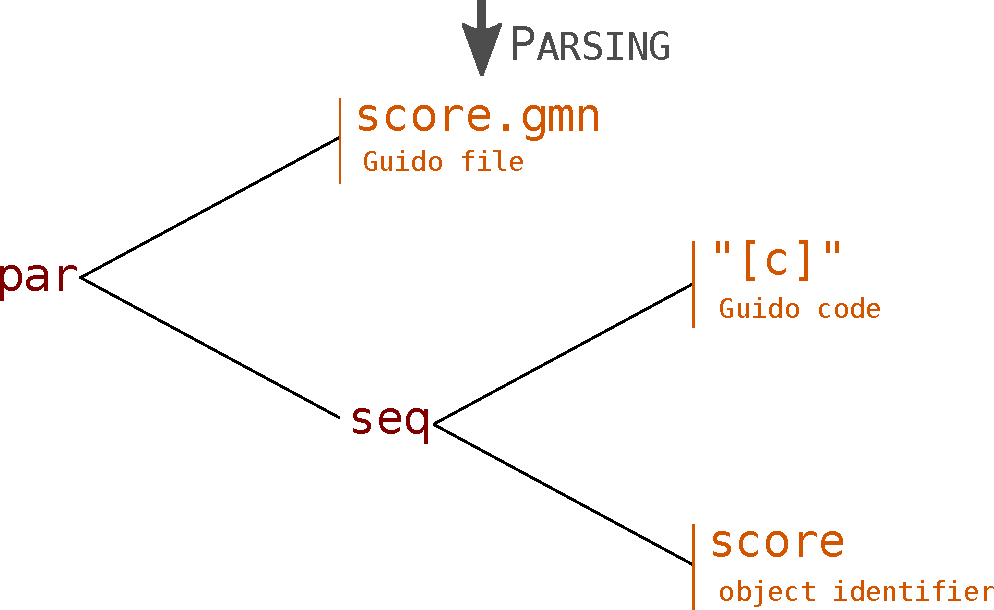
\includegraphics[width=0.9\columnwidth]{imgs/exprParse}
\caption{Parsing \sExpr into its tree form.
\label{fig:example}}
\end{figure}

It's in this tree form that expression are stored, manipulated, assembled and evaluated by INScore. Of course, each node of the tree is an operator and each leather is one argument. Through the process of standard evaluation, each of the leather are interpreted and reduced to guido code which can then be used as arguments for GuidoAR operators. Because one expression can be evaluated in many different ways (in general the result of the evaluation is the corresponding guido code, but it can also be a transcription of the expression in its textual form...), the informations stored in the tree are the exact copy of those contained in the expression string. Type specification of arguments is the only difference, whereas type are implicit in \sExpr, arguments are explicitly stored as Guido code or file or identifier... in the tree form.


\subsubsection{Dynamic evaluation of \sExpr}

In the earlier development of the project the \sExpr used to define an INScore object was parsed, evaluated and the tree was immediately deleted, leaving the newly born object orphan of its history. It was, then, impossible to retrieve its initial definition, and the only way to update its value was to create it again, using the same expression. To solve this performance and ergonomic issue a dynamic evaluation mechanism was introduced.

Each INScore object definable using \sExpr (score or piano roll) had been extended with a \sExpr handler that can store and evaluate  its expression tree. The user can then, whenever he wants, asks the handler to evaluate the expression again, updating the evaluated value if any objects or file changed since the previous evaluation. This process is not automatic, in order to avoid any recursive definition problems as explained in the previous section.

However, as re-evaluate a entire expression can take quite some times, and because, in a context of a real-time score viewer we don't have that time, only the branch that are likely to change are re-evaluated. Indeed, guido or music xml code have no reason to change through time, thus their values should only be evaluated once and kept as they are, these arguments shall be evaluated statically. For the same reason, an operators applied on two statically evaluated node is considered statically evaluated too. After evaluating these nodes, their value is stored together with the expression tree so it can be retrieved afterwards.

Actually, by default all arguments are considered statically evaluated, to state to INScore that a reference to an object or to a file should be evaluated dynamically, one should prefix the argument with the '\&' token. When triggering a re-evaluation, the evaluator shall check if these arguments had changed and re-compute their branch if so.

\subsubsection{Expanding \sExpr}

\section{Using score expressions in INScore}
\subsubsection{Declaring \sExpr}
- set \\
- OSC compatible
\subsubsection{New INScore events}

\subsubsection{New INScore commands}

\section{Examples}

\section{Conclusions}
To finish your full-length paper, end it with a conclusion;
and after careful editing and a final spell-cheek,
submit it through the \href{https://easychair.org/conferences/?conf=tenor2016}{\textcolor {magenta} {\underline {EasyChair Submission System}}}. 
\underline{Do not} send papers directly by e-mail.
%
\begin{acknowledgments}
You may acknowledge people, projects, 
funding agencies, etc. 
which can be included after the second-level heading
``Acknowledgments'' (with no numbering).
\end{acknowledgments} 

%%%%%%%%%%%%%%%%%%%%%%%%%%%%%%%%%%%%%%%%%%%%%%%%%%%%%%%%%%%%%%%%%%%%%%%%%%%%%
%bibliography here
\bibliography{../interlude}

%\begin{INScode}
%scoreExpression: 
%		"expr(" operator score score ")"
%      | "expr(" simpleScore ")"
%only inside a score expression context:
%      | "(" operator score score ")"  
%      ;
%               
%score : scoreExpression
%      | simpleScore
%      ;
%      
%simpleScore: GuidoString
%           | MusicXmlString
%           | filepath
%           | "&" filepath
%           | objectIdentifier
%           | "&" objectIdentifier
%           | "~" objectIdentifier
%           ;
%\end{INScode}

\end{document}

%\begin{figure}[t]
%\centering
%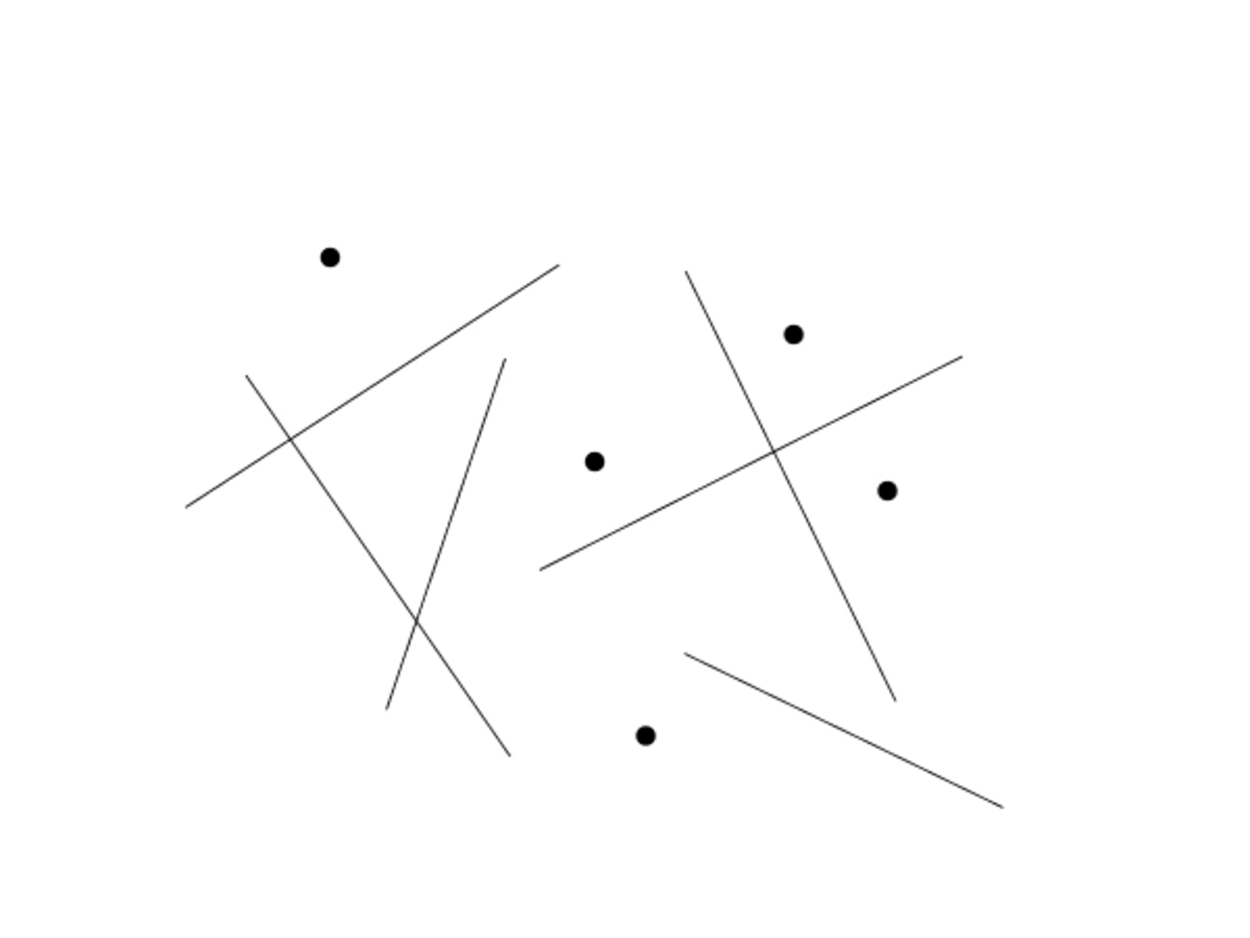
\includegraphics[width=0.9\columnwidth]{figure}
%\caption{Figure captions should be placed below the figure, 
%exactly like this.
%\label{fig:example}}
%\end{figure}

%\begin{figure}[t]
%\figbox{
%\subfloat[][]{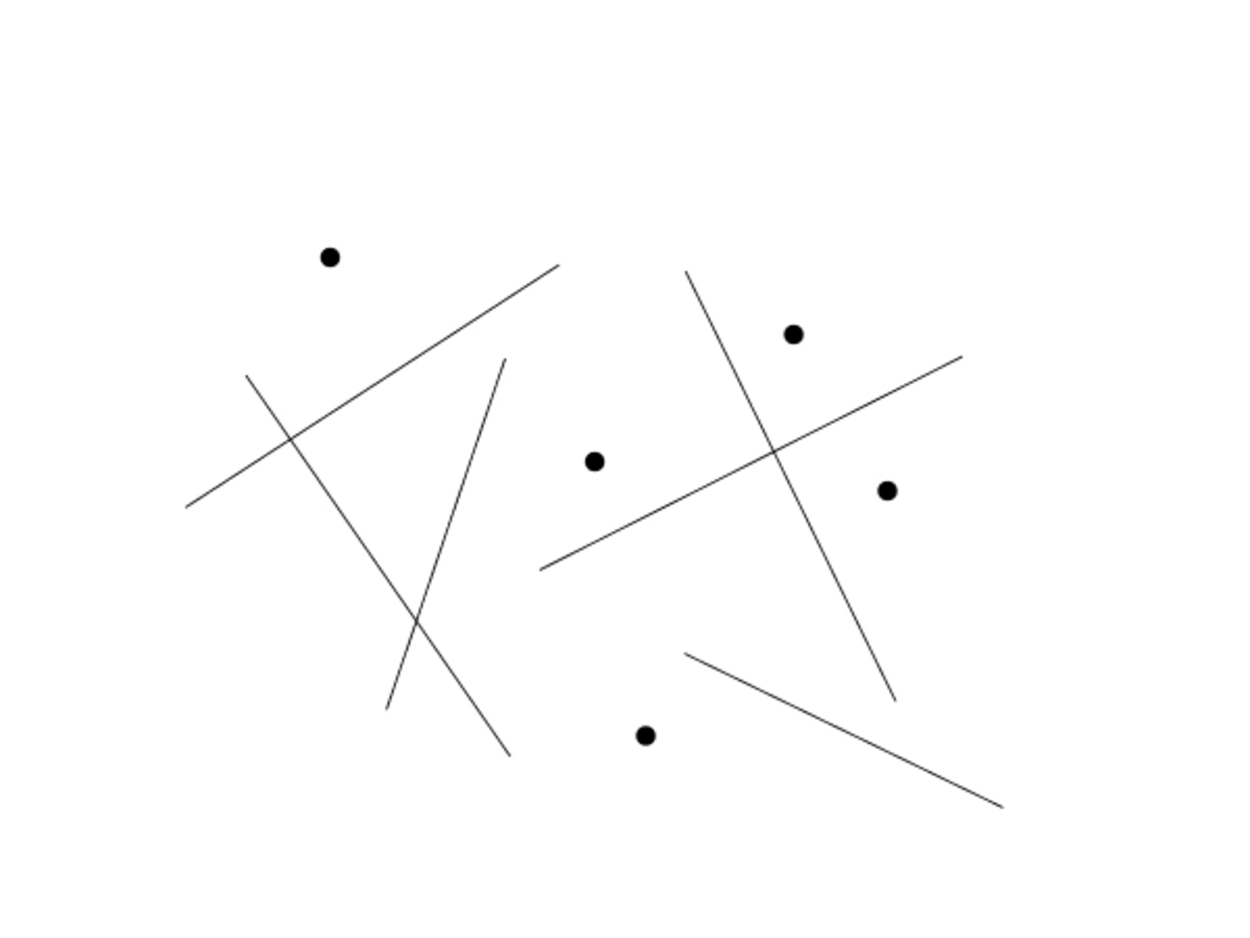
\includegraphics[width=60mm]{figure}\label{fig:subfigex_a}}\\
%\subfloat[][]{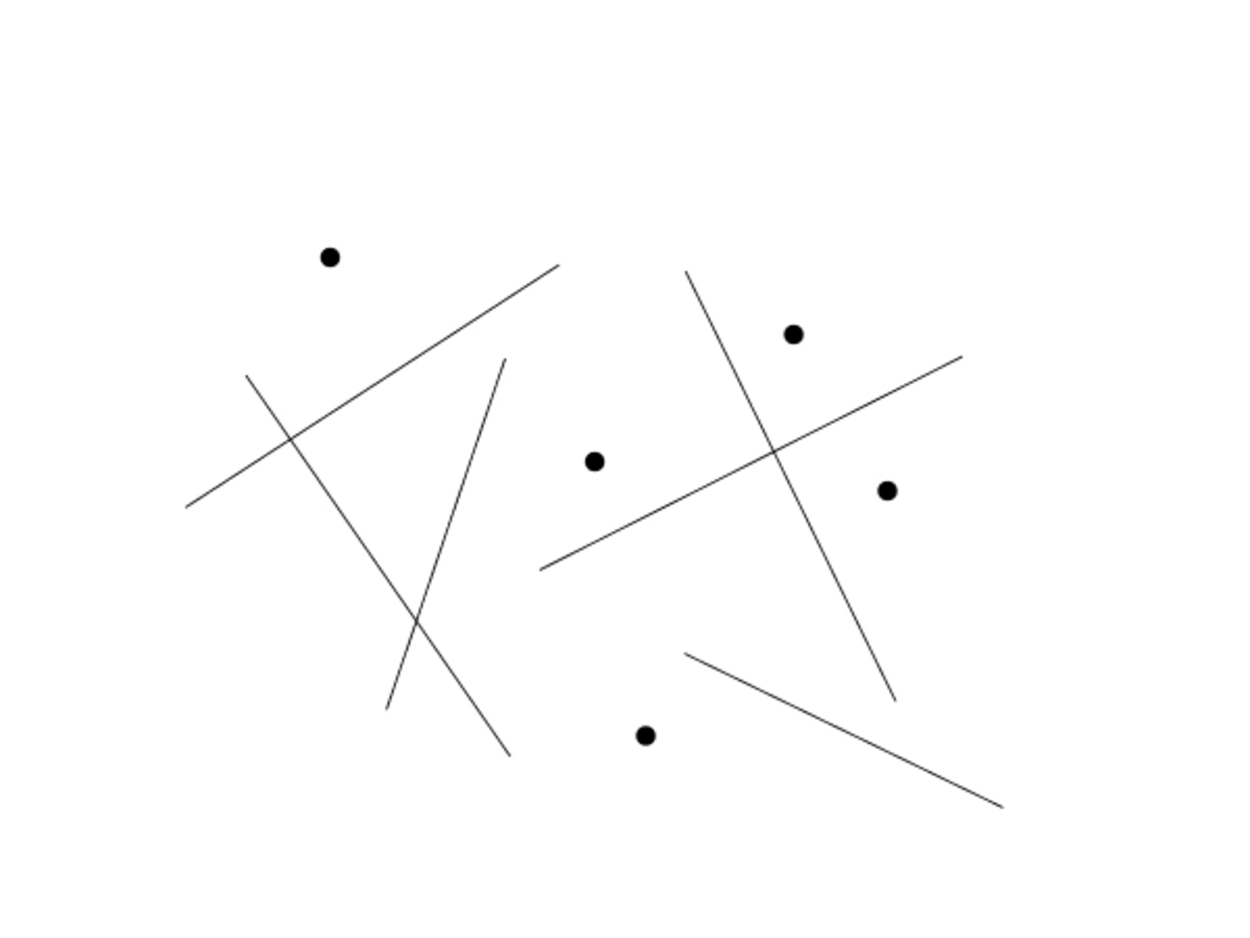
\includegraphics[width=80mm]{figure}\label{fig:subfigex_b}}
%}
%\caption{Here's an example using the subfig package.\label{fig:subfigex} }
%\end{figure}

%\subsection{Footnotes}
%You can indicate footnotes with a number in the text,\footnote{This is a footnote.}
%but try to work the content into the main text.
%Use 8pt font-size for footnotes. 
%Place the footnotes at the bottom of the page 
%on which they appear. 
%Precede the footnote with a 0.5pt horizontal rule.

%\section{Citations}
%List all bibliographical references at the end of your paper,
%inside a section named ``REFERENCES''.
%Order and number the references in order of appearance. 
%Do not list references that do not appear in the text.
%Reference numbers in the text should appear within square brackets, such as 
%in~\cite{Someone:13} or~\cite{Someone:13,Someone:04,Someone:09}.
%The reference format is the standard IEEE one. 
%We highly recommend you use BibTeX 
%to generate the reference list.
